%%%%%%%%%%%%%%%%%%%%%%%%%%%%%%%%%%%%%%%%%%%%%%%%%%%%%%%%%%%%%%%%%%%%
%% I, the copyright holder of this work, release this work into the
%% public domain. This applies worldwide. In some countries this may
%% not be legally possible; if so: I grant anyone the right to use
%% this work for any purpose, without any conditions, unless such
%% conditions are required by law.
%%%%%%%%%%%%%%%%%%%%%%%%%%%%%%%%%%%%%%%%%%%%%%%%%%%%%%%%%%%%%%%%%%%%


\documentclass{beamer}
\usetheme[faculty=fi]{fibeamer}
\usepackage[utf8]{inputenc}
\usepackage[
   main=english, %% By using `czech` or `slovak` as the main locale
                        %% instead of `english`, you can typeset the
                        %% presentation in either Czech or Slovak,
                        %% respectively.
   czech, slovak, greek %% The additional keys allow foreign texts to be
]{babel}            %% typeset as follows:


%% These macros specify information about the presentation
\title{Sampling the flux space of microbial metabolic networks}
\subtitle{the example of SARS-CoV-2 on the human alveolar macrophage metabolic network} %% title page.
\author{Haris Zafeiropoulos} 

%% These additional packages are used within the document:
\usepackage{ragged2e}   % `\justifying` text
\usepackage{booktabs}   % Tables
\usepackage{tabularx}
\usepackage{tikz}         % Diagrams
\usetikzlibrary{calc, shapes, backgrounds}
\usepackage{amsmath, amssymb}
\usepackage{url}          % `\url`s
\usepackage{listings}   % Code listings
\usepackage{setspace}

\frenchspacing

\begin{document}

   \shorthandoff{-}
   \frame[c]{\maketitle}

   % SLIDE 2
   \begin{frame}{Genome-scale metabolic reconstruction}
      
      \begin{singlespace}
         \begin{tikzpicture}[overlay,remember picture]
            \node[anchor=north west, xshift=30pt,yshift=-50pt]
               at (current page.north west) {
                  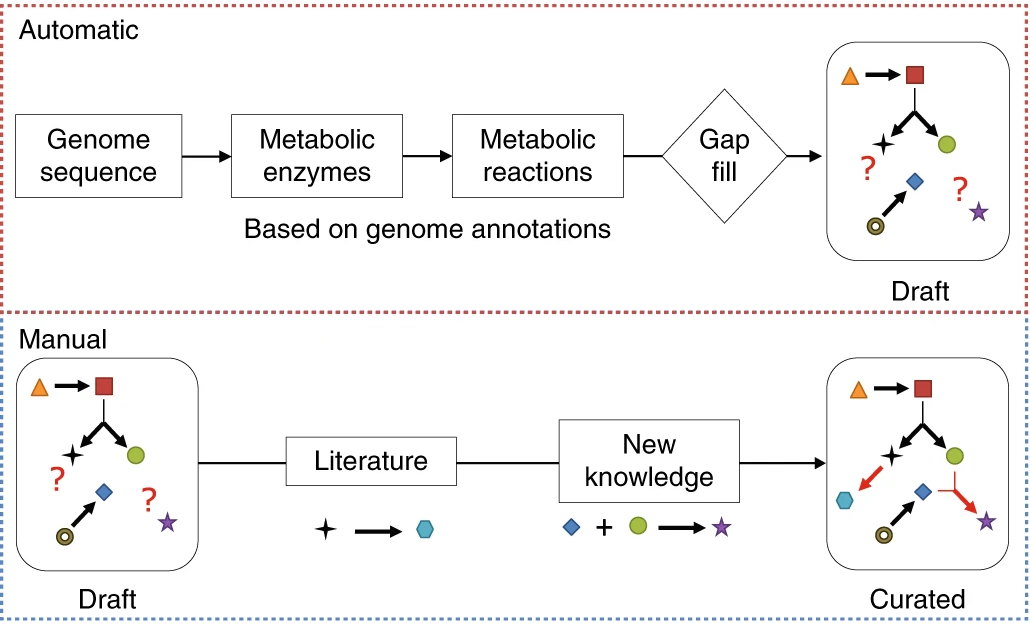
\includegraphics[width=105mm]{../resources/building_gmd_transparent.png}
               };
            \node[align = left, above, yshift=10] at (current page.south) {
               \scriptsize 
               Figure from: Heirendt, Laurent, et al. Nature protocols 14.3 (2019): 639-702.
            };
         \end{tikzpicture}
      \end{singlespace}
      % \captionof{figure}{\textbf{Confusion Matrix}}

   \end{frame}
   
   % SLIDE 3
   \begin{frame}{From a stoichiometric matrix}
      \framesubtitle{to a constraint-based model}
      
      \begin{singlespace}
         \begin{tikzpicture}[overlay,remember picture]

            \node[anchor=north west, xshift=20pt,yshift=-65pt]
               at (current page.north west) {
                  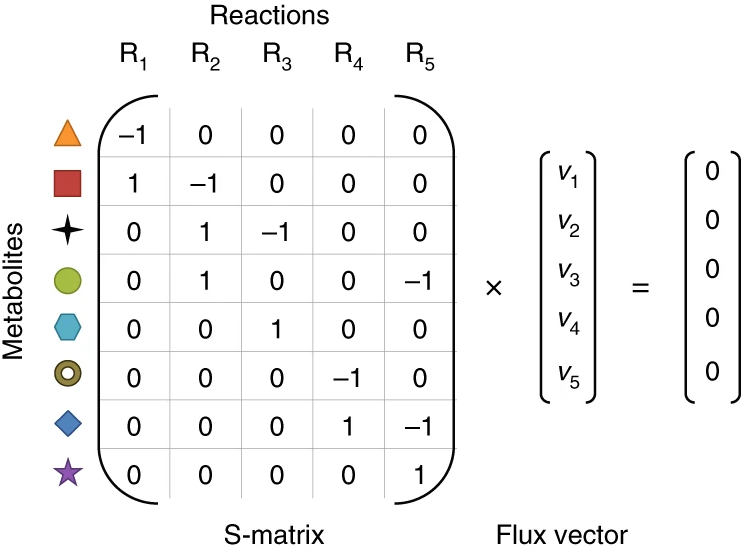
\includegraphics[width=70mm]{../resources/stoichiometric_matrix_transparent.png}
               };

               \node[align = left, above, yshift=10] at (current page.south) {
                  \scriptsize 
                  Figure from: Heirendt, Laurent, et al. Nature protocols 14.3 (2019): 639-702.
               };
   
            \node[align = center, left, xshift=-10pt] at (current page.east) {
               \small
               \textbf{Flux Balance Analysis}
               \\ 
               \small
               Maximize \/ minimize an \\
               \small
               objective function:  \\
               \small
               $\psi = c_1 v_1 + c_2 v_2 + .. + c_5 v_5$ \\
               \small
               such that: \\
               \small
               $S * v = O$ \\ 
               \small
               and for each reaction $i$: \\
               \small
               $lb_i <= v_i <= ub_i$ \\ 
               
               \\

               \small
               where $lb$: lower bound, \\
               \small
               $ub$: upper bound and \\
               \small
               $S$: the stoichiometric matrix
            };

         \end{tikzpicture}
      \end{singlespace}      
   \end{frame}


   % SLIDE 4
   \begin{frame}[label=simmonshall]{Flux sampling} 

      \framesubtitle{an alternative approach}
      \begin{singlespace}
         \begin{tikzpicture}[overlay,remember picture]

            \node[anchor=north west, xshift=30pt,yshift=-60pt]
               at (current page.north west) {
                  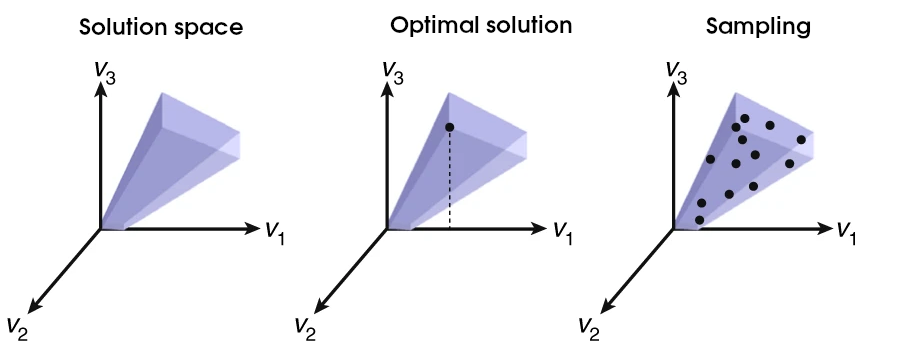
\includegraphics[width=100mm]{../resources/solution_spaces_transparent.png}
               };

               \node[align = left, above, yshift=10] at (current page.south) {
                  \scriptsize 
                  Figure from: Heirendt, Laurent, et al. Nature protocols 14.3 (2019): 639-702.
               };

            \end{tikzpicture}

         \bigskip  \justifying  \bigskip
         \bigskip  \justifying  \bigskip
         \bigskip  \justifying  \bigskip

            \begin{itemize}
               \item \small 
               enables the analysis of GSMMs without the need of an objective function
               \item \small
               determines the feasible solution spaces for fluxes in a network based on a set of conditions as well as the probability of obtaining a solution               
            \end{itemize}

      \end{singlespace}
   \end{frame}
 

   % SLIDE 5
   \begin{frame}{Our Markov Chain Monte Carlo (MCMC) algorithm}
      \framesubtitle{for flux sampling}

      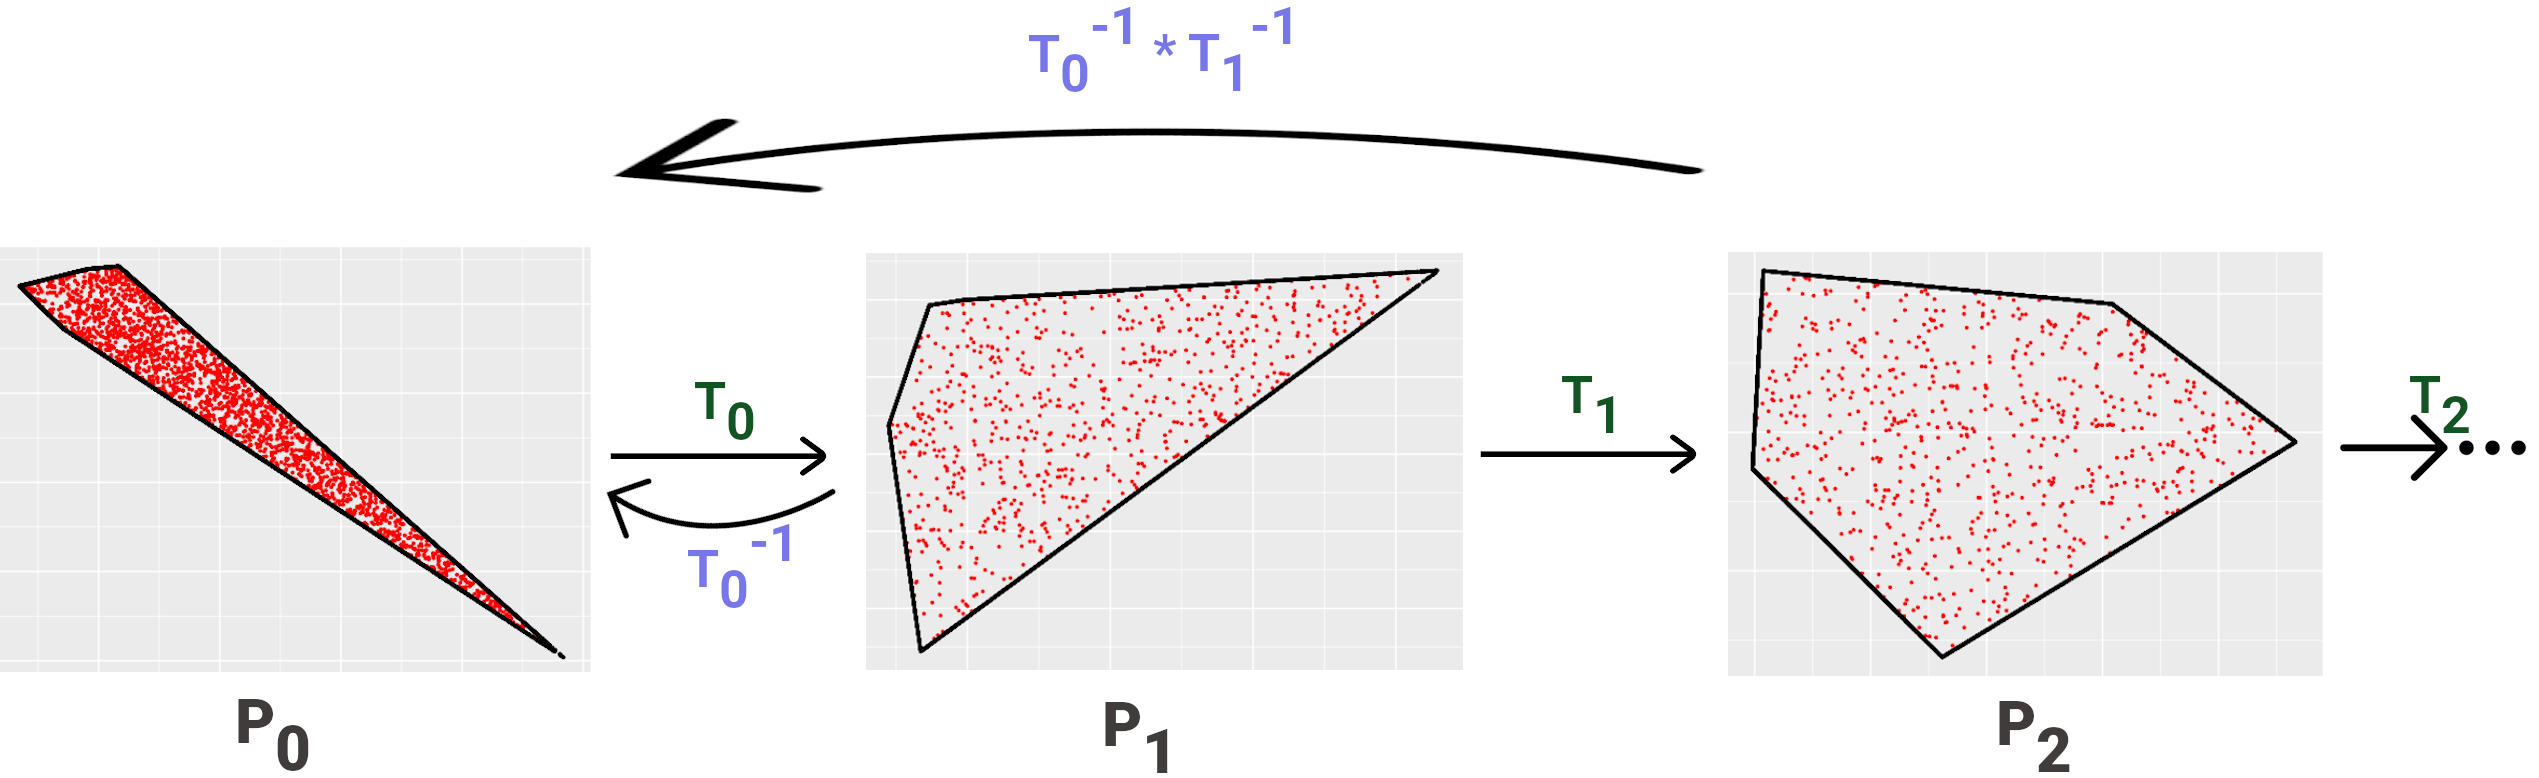
\includegraphics[scale=0.11]{../resources/sampling_extra_phase_croped_transparent.png}
      
      \scriptsize
      \begin{block}{Steps of an MMCS phase}
         \begin{itemize}
            \item \textbf{sampling step:} using a variant of the \textbf{Billiard walk}  
            \item \textbf{rounding step:} calculate a linear transformation $T_i$ that puts the sample into isotropic position and then apply it on $P_i$ to obtain the polytope of the next phase
            \item check several statistic tests
         \end{itemize}      

      \end{block}

      \begin{singlespace}
         \scriptsize
         Chalkis, Fisikopoulos, Tsigaridas and Zafeiropoulos 
         "Geometric Algorithms for Sampling \\ the Flux Space
         of Metabolic Networks", SoCG 2021,  
         DOI: 10.4230/LIPIcs.SoCG.2021.21
   
      \end{singlespace}

   \end{frame}


   % SLIDE 6
   \begin{frame}{Find possible anti-COVID19 targets}
      \framesubtitle{a flux sampling application}
      \bigskip
      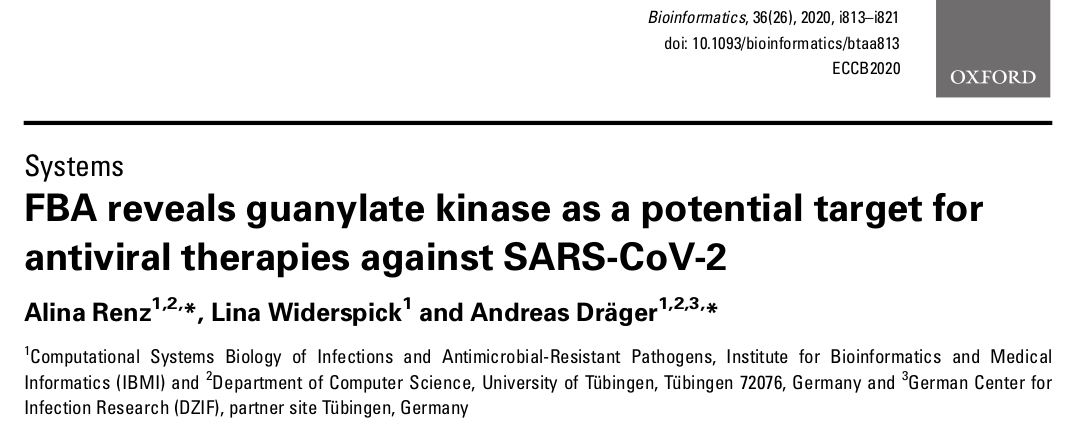
\includegraphics[scale=0.27]{../resources/covid_paper.png}
      
      \begin{singlespace}
         \begin{itemize}
            \item \small Renz et al. '20 built the biomass function of Sars-Cov-2 to build a host - virus network
            \item \small Using FBA they computed an optimal steady state using \\ \small \quad (i) human biomass maintenance,\\ \small \quad (ii) virus growth rate
            \item \small They found reaction GK1 as a possible anti-viral target.
         \end{itemize}            
      \end{singlespace}

   \end{frame}

   % SLIDE 7
   \begin{frame}{Find possible anti-COVID19 targets}
      \framesubtitle{a flux sampling application}      

      \centerline{
      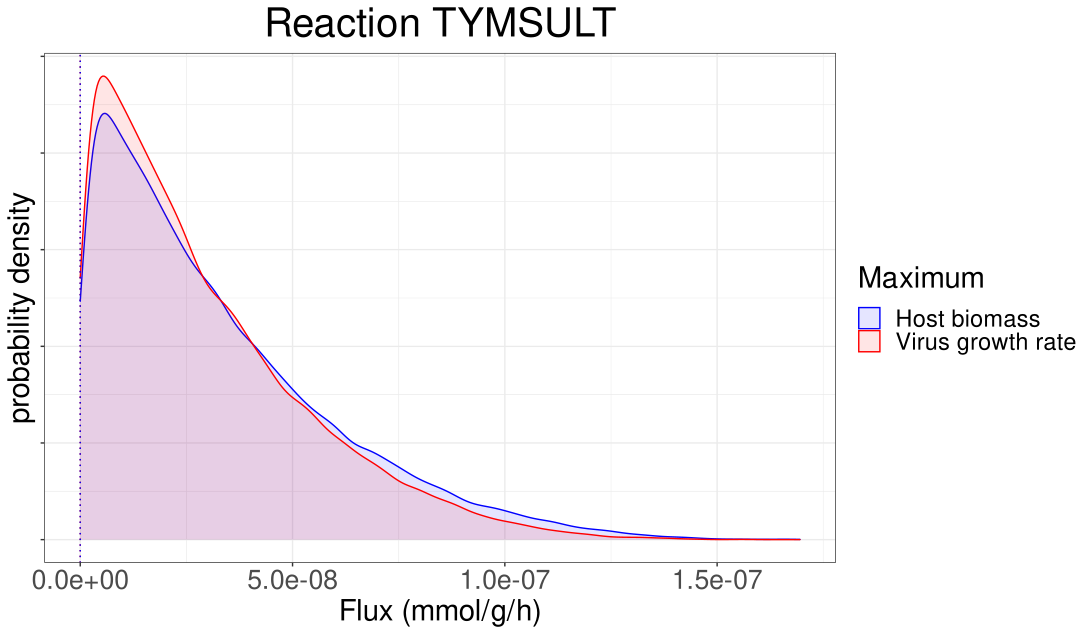
\includegraphics[scale=0.21]{
         ../resources/density_flux_TYMSULT_fba_2_transparent
         } 
      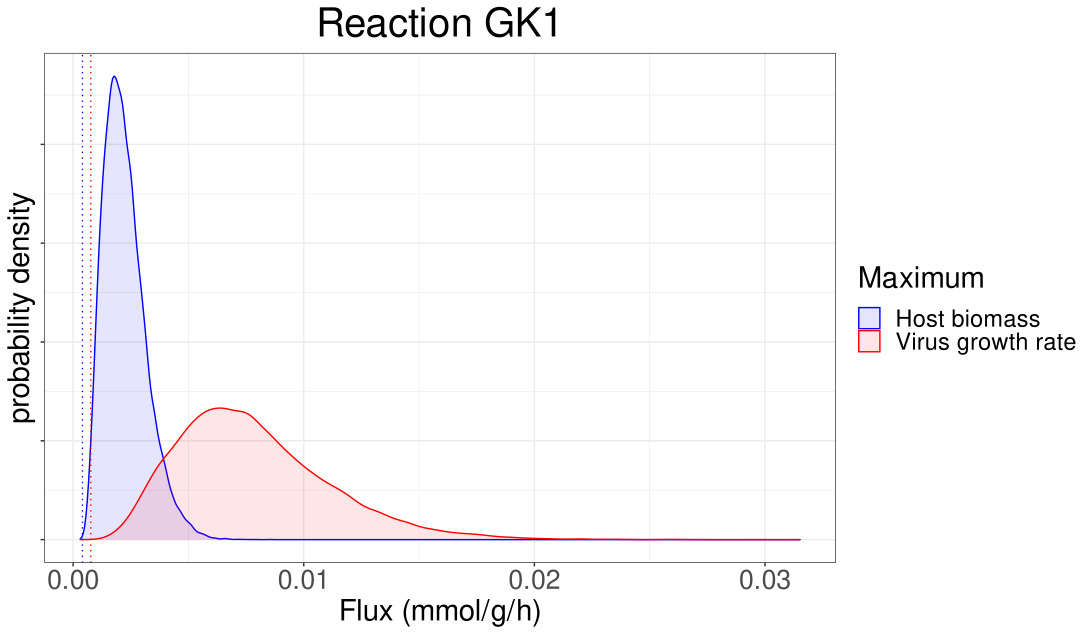
\includegraphics[scale=0.21]{
         ../resources/density_flux_gk1_fba_2_transparent
         }
      }

      \begin{itemize}
         \item Check if the flux distribution of a reaction changes.
         \item Find possible anti-viral targets and study further..
      \end{itemize}
      \vspace*{0.2cm}

   \end{frame}
   

   % % SLIDE 8
   % \begin{frame}{Further applications}
   %    \framesubtitle{of metabolic flux sampling}
      
   %    \begin{tikzpicture}[overlay,remember picture]

   %       \node[anchor=north west]
   %       at (current. page.nort west) {
   %          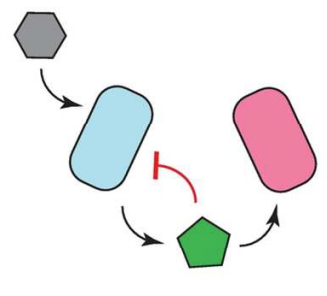
\includegraphics[width=40mm]{../resources/interactions.png}

            
   %       }
         
   %       \node[anchor=north east, xshift=00pt,yshift=-100pt]
   %       at (current page.north east) {
   %          
\includegraphics[width=55mm]{../resources/cartoon_wine}
   %       };

   %    \end{tikzpicture}

   % \end{frame}


   % SLIDE 9 - Thank you SLIDE
   \begin{darkframes}
   \begin{frame}{Thank you for your attention}
         
      % URLs
      GitHub repository  : \href{https://github.com/GeomScale/dingo/}{https://github.com/GeomScale/dingo/} \\ 

      MMCS algorithm publication: \href{10.4230/LIPIcs.SoCG.2021.21}{10.4230/LIPIcs.SoCG.2021.21} \\ 
      
      \bigskip
      email    : \href{haris-zaf@hcmr.gr}{haris-zaf@hcmr.gr} \\
      Twitter  : \href{https://twitter.com/haris_zaf}{haris\_zaf} \\
      web-site : \url{https://hariszaf.github.io/} \\

      % Logos   
      % -------------- 

      % UoC
      \begin{tikzpicture}[overlay,remember picture]
         \node[anchor=south west,
               xshift=-350pt,
               yshift=10pt]
               at (current page.south east) {
                  
\includegraphics[height=17mm]{
                     ../resources/UoC_logo_white.png
                  }
               };
      \end{tikzpicture}

      % IMBBC
      \begin{tikzpicture}[overlay,remember picture]
         \node[anchor=south east,
            xshift=-185pt,
            yshift=25pt]
            at (current page.south east) {
               
\includegraphics[width=35mm]{../resources/logo-imbbc.png}
            };
      \end{tikzpicture}%

      % HCMR
      \begin{tikzpicture}[overlay,remember picture]
         \node[anchor=south east,
               xshift=-125pt,
               yshift=10pt]
               at (current page.south east) {
                  
\includegraphics[height=20mm]{
                     ../resources/hcmr-logo.png
                  }
               };
      \end{tikzpicture}%

      % GeomScale
      \begin{tikzpicture}[overlay,remember picture]
         \node[anchor=south east,
               xshift=-5pt,
               yshift=22pt]
               at (current page.south east) {
                  
\includegraphics[width=40mm]{
                     ../resources/geomscale-logo.png
                  }
               };
      \end{tikzpicture}

   \end{frame}
   \end{darkframes}

\end{document}
